% Tämä on fysiikan laboratoriotöiden selostuspohjapohja.
% Pohja ei kuitenkaan ole mikään virallinen ja oikea totuus, 
% eli muistakin pohjia voi käyttää. Tämän tarkoitus on ainoastaan 
% auttaa opiskelijoita LaTeXin alkuun.
%
% Pohjaa saa levittää ja muuttaa vapaasti. Pohjan muuttajan toivotaan 
% kuitenkin lisäävän tiedot muutoksesta ja sen ajankohdasta tämän 
% kommenttiosuuden loppuun.  
%
% Pikainen käyttöohje:
% Päivita kansilehden tiedot
% Kirjoita selostuksesi
% ATK-keskuksessa käännät koodin seuraavilla komennoilla:
% use latex
% latex selkkari.tex
% 
% Esikatsele:
% xdvi selkkari
%
% Possuksi (tiedostonimeksi selostus.ps):
% dvips -o selostus.ps selkkari
%
% Toivottavasti tämä pohja auttaa alkuun
%
% Jukka Katainen, 6.2.2004
%
\documentclass[a4paper,11pt]{article}

\frenchspacing
\usepackage[finnish]{babel}
\usepackage[utf8]{inputenc}
\usepackage{graphicx}
\usepackage[T1]{fontenc}
\usepackage{float}
\usepackage{gensymb}

\begin{document}

%Tästä alkaa selkkarin kansilehti. Vaihda tilalle tarvittavat tiedot.
\begin{titlepage}
\pagestyle{empty}
\begin{center}

\vspace*{3cm}
\noindent\LARGE{\textbf{Työ 
%
%*******************************************************
%Työn numero:
14
%*******************************************************
%
\\
%
%*******************************************************
%Työn nimi:
Lämmönjohtavuus
%*******************************************************
%
}}\\
\vspace*{2cm}
Työvuoro \LARGE{\textbf{
%
%*******************************************************
%Työvuoro:
51
%*******************************************************
%
}} pari \LARGE{\textbf{
%
%*******************************************************
%Parin numero:
4
%*******************************************************
}}\\
\vspace*{1cm}
\large{
\begin{tabular}{l l}
%
%*******************************************************
%Parin opiskelijat ja opiskelijanumerot:
Juho Salmii & 80391C\\
Jukka Kemppainen & \\
%*******************************************************
%
\end{tabular}

\vspace*{1cm}
Selostuksen laati \emph{
%
%*******************************************************
% Selostuksen tekijä:
Juho Salmi
%*******************************************************
%
} \\
\vspace*{1cm}
\begin{tabular}{l l}
Mittaukset suoritettu & \textbf{
%
%*******************************************************
% Mittaukset suoritettu
25.11.2013
%*******************************************************
%
}\\
Selostus palautettu & \textbf{
%
%*******************************************************
% Selostus palautettu
2.12.2013
%*******************************************************
%
}\\
\end{tabular}
}
\end{center}
\end{titlepage}
%kansilehti loppuu tähän

%Varsinainan selkkari alkaa
\section{Johdanto}

Lämpöenergia on kineettistä energiaa hiukkastasolla. Lämmönjohtuminen tapahtuu, kun energia siirty hiukkaselta toiselle. Johtumista tapahtuu myös vapaasti hilassa liikkuvien elektronien diffuusion välityksellä. Eri aineilla on erilainen lämmönjohtavuus. Tässä työssä tutkitaan lämmönjohtavuutta erilaisissa materiaaleissa. \cite{wiki:thermal}

\section{Laitteisto ja menetelmät}

Työssä käytetään kuvassa \ref{laitteisto} esitettyä laitteistoa. Höyrygeneraattorilla tuotetaan 100\degree C vesihöyryä, josta se johdetaan höyrykammioon. Höyrykammion päälle asetetaan levy, jonka lämmönjohtavuuden ominaisuuksia tutkitaan. Levyn päälle asetetaan jääpala, jonka sulamisesta päätellään levyn lämmönjohtavuus. Jääpalan pinta on 0\degree C, joten lämpötilaero levyn puolien välillä on 100K. Tässä työssä tehdään mittaukset polykarbonaattilevylle sekä kahdelle lasilevylle. 

\begin{figure}[H]
\centering 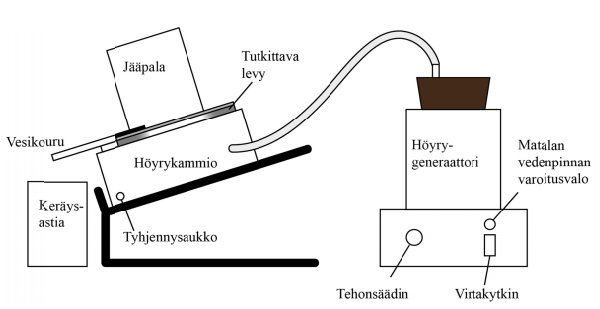
\includegraphics[width=0.8\textwidth]{laitteisto}
\caption{Työssä käytetty laitteisto. \label{laitteisto}}
\end{figure}

Lämpövirtaus on kääntäen verrannollinen lämpöä eristävän kerroksen paksuuteen

\begin{equation}
  \label{lampovirtaus}
  \frac{\Delta Q}{\Delta t} = k A \frac{T_1 - T_2}{l} ,
\end{equation}

missä $\Delta Q$ on kerroksen läpi siirtynyt lämpömäärä ja, A pinta-ala $T_1 - T_2$ lämpötilaero, $l$ paksuus ja $k$ lämmönjohtavuuskerroin. 

Useampaa päällekkäisen kerroksen tapauksessa lasketaan niiden yhteenlasketut ominaisuudet seuraavasti: 

\begin{equation}
  \Delta T_{tot} = \sum_{i=1}^N (T_i - T_{i-1})
\end{equation}

\begin{equation}
  l_{tot} = \sum_{i=1}^N l_i
\end{equation}

\begin{equation}
  \label{kerrosjohtavuus}
  \frac{l_{tot}}{k_{tot}} = \sum_{i=1}^N \frac{l_i}{k_i}
\end{equation}

\begin{equation}
  \frac{\Delta Q}{\Delta t} = k_{tot} A \frac{\Delta T_{tot}}{l_{tot}} ,
\end{equation}

\section{Tulokset}

Mitataan työssä käytettävien levyjen paksuus. 
\begin{table}[H]
\begin{center}
\caption{Mittaukset levyjen paksuuksista.}
\begin{tabular}{ | r | r | r | }
  \hline 
  Lasilevyn 1 paksuus (mm) & Lasilevyn 2 paksuus & Polykarbonaattilevyn paksuus (mm) \\ \hline
  5,62 & 5,585 & 5,37 \\ \hline
  5,615 & 5,585 & 5,37 \\ \hline
  5,62 & 5,585 & 5,38 \\ \hline
  5,615 & 5,59 & 5,36 \\ \hline
  5,61 & 5,595 & 5,37 \\ \hline
  keskiarvo: 5,616 & keskiarvo: 5,579 & keskiarvo: 5,37 \\ \hline
\end{tabular}
\end{center}
\end{table}

Tehdään mittaukset levyjen lämmönjohtavuuksien mittaamiseksi. Mitataan jääpalan halkaisija ennen ja jälkeen mittauksen, otetaan aika, jonka jääpala sulaa levyn päällä sekä mitataan sulamisveden massa.
\begin{table}[H]
\begin{center}
\caption{Mittaustulokset lämmönjohtavuuksien mittaamiseksi.}
\begin{tabular}{ | p{2.5cm} | p{2.5cm} | p{2.5cm} | p{2.5cm} | p{2.5cm} | }
  \hline 
  Mitattava levy & Veden keräysaika (s) & Kerätyn veden massa (g) & Jääpalan halkaisija aluksi (mm) & Jääpalan halkaisija lopuksi (mm) \\ \hline
  Lasi 1 & 183 & 31 & $60 \pm 5$ & $57 \pm 5$ \\ \hline
  Polykarbonaatti & 654 & 29,4 & $57 \pm 5$ & $53 \pm 5$ \\ \hline
  Lasi 2 + polykarbonaatti & 1021 & 28,51 & $53 \pm 5$ & $50 \pm 5$ \\ \hline
\end{tabular}
\end{center}
\end{table}

Arvioidaan virheet. Ajan virheeksi arvioidaan 1 s sillä pyöristimme ajan sekunnin tarkkuuteen. Massan virheeksi arvioidaan vaa'an hyvästä tarkkuudesta huolimatta 0,5 g, sillä osa vedestä menee hukkaan mittaus prosessissa. Halkaisijan virheeksi arvioidaan 5 mm, sillä jääpala oli epämääräisen muotoinen ja sitä oli liukkauden takia vaikea mitata. 

Johdetaan kaavasta \ref{lampovirtaus} seuraava kaava, jolla voidaan laskea lasilevyn lämmönjohtavuuskerroin: 

\begin{equation}
  k = \frac{m \cdot C_s \cdot l}{t \cdot A \cdot (T_2 - T_1)} ,
\end{equation}

Missä $m$ on kerätyn veden massa, $C_s$ veden sulamislämpö, $t$ keräysaika ja $A$ jääpalan pohjan pinta-ala. 

Määritetään lasilevy 1:n lämmönjohtavuus seuraavan taulukon avulla. 
\begin{table}[H]
\begin{center}
\caption{Lukuarvot lasilevy 1:n lämmönjohtavuuden määrittämiseksi. }
\begin{tabular}{ | p{3cm} | p{3cm} | p{3cm} | p{3cm} | }
  \hline 
  Suure & Arvo & Virhe & Yksikkö \\ \hline
  Jään halkaisija & 60 & $\pm 5$ & mm \\ \hline
  Levyn paksuus keskiarvona & 5,616 & $\pm 0,1$ & mm \\ \hline
  Lämpötilaero & 100 & $\pm 1$ & K \\ \hline
  Veden sulamislämpö & 333 & & kJ/kg \\ \hline
  Lasin lämmönjohtavuus & 1,212 & $\pm 0,018$ & W/Km \\ \hline
\end{tabular}
\end{center}
\end{table}

Virhelähteitä vertailemalla huomataan, että veden massan virhe osuus kokonaisvirheestä on n. 99 \%. Jään halkaisijan osuus virheestä on 1 \% ja lasilevyn paksuuden sekä sulamisajan osuudet ovat edellisiin nähden merkityksettömiä. 
   
Määritetään vastaavasti polykarbonaattilevyn sekä kerrosrakenteen lämmönjohtavuus. Saadaan polykarbonaattilevyn lämmönjohtavuudeksi 0,345 W/Km ja kerrosrakenteen lämmönjohtavuudeksi 0,482 W/Km. 

Kaavasta \ref{kerrosjohtavuus} johdettuna tulokseksi olisi pitänyt tulla 0,520 W/Km. Tulokset ovat samaa suuruusluokkaa, ja eroa selittää levyjen väliin jäänyt ohut ilmakerros. 

\section{Yhteenveto ja pohdinnat}

Mittausmenetelmä ei sovellu tarkkaan lämmönjohtavuuden mittaukseen, mutta antaa suuntaa siitä, kuinka hyvin eri materiaalit lämpöä eristävät. 

Virheitä mittauksissa vältettäisiin parhaiten eristämällä mittaus paremmin. Pitää estää, että vettä haihtuu ja kuluu siirroissa astiasta toiseen. Veden voisi johtaa esim. paremmin suljettuun pulloon, jota punnitaan suoraan vaa'alla. 

Samoin jääpala pitäisi eristää paremmin, sillä siihen tulee lämpöä myös muualta ympäristöstä. Tämä aiheuttaa sen, että saadut lämmönjohtavuudet ovat suurempia kuin levyjen todelliset lämmönjohtavuudet. 

%Kirjallisuuviitteet
\begin{thebibliography}{99}
% Kirjallisuus viitteet tähän tapaan:
%\item{R.W. Robinnet, Quantum Mechanics, Oxford University Press, 1997}

\bibitem{ohje} Harjoitustyöohje: Työ 14 Lämmönjohtavuus, http://physics.aalto.fi/pub/kurssit/Tfy-3.15xx/materiaali/14.pdf [Viitattu 18.11.2013]
\bibitem{wiki:thermal} Wikipedia-artikkeli lämmönjohtavuudesta, http://en.wikipedia.org/wiki/Thermal\_conduction [Viitattu 2.12.2013]

\end{thebibliography}

%liitteet numeroituna
\section*{Liitteet}
\begin{enumerate}
%Liitteet tähän tapaan
\item{Mittauspöytäkirja}\label{mittaus}

\end{enumerate}

\end{document}
